% =====================================================================
%  Métodos Matemáticos para Ciencias Físicas
%  Trabajo de investigación complementario — Tema 2
%  Propagación de ondas electromagnéticas en medios disipativos
%  y el teorema de los residuos
%
%  Compilar:  pdflatex tema2.tex  (dos veces, para referencias cruzadas)
%  Las figuras 1 y 3 se generan con  python3 figuras/generar_figuras.py
% =====================================================================
\documentclass[11pt,letterpaper]{article}

% ---------- Idioma y tipografía ----------
\usepackage[T1]{fontenc}
\usepackage[utf8]{inputenc}
\usepackage[spanish,es-nodecimaldot,es-noquoting]{babel}
\usepackage{mathpazo}            % Palatino + matemáticas Pazo
\usepackage{microtype}

% ---------- Matemáticas ----------
\usepackage{amsmath,amssymb}
\usepackage{bm}

% ---------- Página ----------
\usepackage[letterpaper,margin=1in,headheight=14pt]{geometry}
\usepackage{fancyhdr}
\usepackage{xcolor}
\usepackage{graphicx}
\usepackage{subcaption}
\usepackage[font=small,labelfont=bf,labelsep=period]{caption}
\usepackage{titlesec}
\usepackage{enumitem}
\usepackage[breakable,skins]{tcolorbox}
\usepackage{tikz}
\usetikzlibrary{arrows.meta,decorations.markings}
\usepackage[hidelinks]{hyperref}

% ---------- Colores ----------
\definecolor{azul}{HTML}{1F5FBF}
\definecolor{naranja}{HTML}{E8603C}
\definecolor{fondo}{HTML}{F3F2EE}
\hypersetup{colorlinks=true,linkcolor=azul,citecolor=azul,urlcolor=azul}

% ---------- Encabezados ----------
\pagestyle{fancy}
\fancyhf{}
\fancyhead[L]{\color{black!70}Tema 2 $\cdot$ Ondas electromagnéticas y teorema de los residuos}
\fancyhead[R]{\thepage}
\renewcommand{\headrulewidth}{0.4pt}

% ---------- Títulos de sección ----------
\titleformat{\section}{\large\bfseries\color{azul}}{\thesection.}{0.5em}{}
\titleformat{\subsection}{\normalsize\bfseries}{\thesubsection}{0.6em}{}
\titlespacing*{\section}{0pt}{2.0ex plus .5ex}{1.0ex}
\titlespacing*{\subsection}{0pt}{1.6ex plus .4ex}{0.6ex}

% ---------- Listas ----------
\setlist[itemize]{label={\scriptsize$\blacksquare$},leftmargin=1.6em,itemsep=2pt}

% ---------- Cajas de ejemplos ----------
\newcounter{ejemplo}
\newtcolorbox{ejemplobox}{enhanced,breakable,colback=fondo,colframe=fondo,
  borderline west={2.5pt}{0pt}{azul},arc=0pt,outer arc=0pt,
  left=8pt,right=8pt,top=6pt,bottom=6pt,before skip=8pt,after skip=8pt}
\newenvironment{ejemplo}[1]{%
  \refstepcounter{ejemplo}%
  \begin{ejemplobox}\textbf{Ejemplo~\theejemplo\ (#1).}\ }%
  {\end{ejemplobox}}
\newenvironment{nota}{\begin{ejemplobox}}{\end{ejemplobox}}

% ---------- Macros ----------
\newcommand{\dd}{\mathrm{d}}
\newcommand{\nh}{\hat{n}}
\newcommand{\kh}{\hat{k}}
\newcommand{\eps}{\varepsilon}
\DeclareMathOperator{\Res}{Res}
\renewcommand{\Re}{\operatorname{Re}}
\renewcommand{\Im}{\operatorname{Im}}
\newcommand{\vp}{P}   % valor principal de Cauchy

\setlength{\parindent}{1.5em}
\linespread{1.0}

% =====================================================================
\begin{document}

% --------------------------- Portada ---------------------------------
\begin{titlepage}
  \centering
  \vspace*{3.2cm}
  {\textsc{Métodos Matemáticos para Ciencias Físicas}\par}
  \vspace{0.4cm}
  {Trabajo de investigación complementario\par}
  \vspace{2.6cm}
  \rule{0.8\textwidth}{0.4pt}\par
  \vspace{0.7cm}
  {\LARGE\bfseries Propagación de ondas electromagnéticas\\[0.25em]
   en medios disipativos y el\\[0.25em] teorema de los residuos\par}
  \vspace{0.6cm}
  \rule{0.8\textwidth}{0.4pt}\par
  \vspace{0.6cm}
  {\large Tema 2\par}
  \vspace{0.15cm}
  {\small\itshape Variable compleja, integración de contorno, índice de
   refracción complejo, ley de Snell compleja, reflexión y transmisión en
   interfaces, reflexión total interna atenuada y plasmónica de superficie\par}
  \vfill
  {\large\bfseries María Santamaría\par}
  \vspace{0.4cm}
  {Fecha de entrega: 25 de noviembre de 2026\par}
  \vspace{2.2cm}
\end{titlepage}
\setcounter{page}{1}

% --------------------------- Resumen ---------------------------------
\begin{quote}
\small
\textbf{Resumen.} Cuando una onda electromagnética viaja por un medio que
absorbe energía, la permitividad, el índice de refracción y el vector de onda
dejan de ser números reales. Este trabajo muestra que esa
``complejización'' no es un artificio: convierte a la variable compleja en la
herramienta natural del problema. Con el teorema de los residuos se calculan
integrales de dispersión, se prueba que la respuesta de un medio es causal y
se deducen las relaciones de Kramers--Kronig, que ligan la refracción con la
absorción. Luego se estudia la ley de Snell con índice complejo, los
coeficientes de Fresnel, la reflexión total interna atenuada y los plasmones
de superficie, que aparecen como un polo del coeficiente de reflexión. Cada
idea se ilustra con ejemplos resueltos y datos del oro a 632.8\,nm.
\end{quote}

% =====================================================================
\section{Introducción}

En el vacío, la luz se propaga sin perder energía y su descripción se hace con
números reales: la amplitud y la fase de un campo armónico. En la materia real
esto deja de ser cierto. Los electrones ligados de un dieléctrico y los
electrones libres de un metal responden al campo con cierto retraso y disipan
parte de la energía en forma de calor. El modo más económico de describir esa
respuesta es permitir que la permitividad relativa
$\eps(\omega)=\eps'+i\eps''$ y el índice de refracción $\nh=n+i\kappa$ sean
complejos: la parte real gobierna la velocidad de fase y la parte imaginaria la
atenuación~\cite{Jackson,BornWolf}.

Una vez que las magnitudes físicas viven en el plano complejo, las herramientas
de la variable compleja dejan de ser un recurso de cálculo y pasan a contener
física. Las integrales de Fourier que conectan el dominio del tiempo con el de
la frecuencia se evalúan cerrando contornos y sumando residuos~\cite{Arfken};
la ubicación de los polos en el plano de la frecuencia expresa si un sistema es
causal; y los ceros y polos de los coeficientes de reflexión corresponden a
fenómenos medibles, como el ángulo de Brewster o las ondas superficiales. Este
último punto tiene una larga historia: ya en 1909 Sommerfeld estudió la
propagación de ondas de radio sobre un suelo conductor deformando contornos de
integración y encontró una contribución de onda superficial asociada a un
polo~\cite{Sommerfeld}. La relación entre causalidad y analiticidad dio origen
a las relaciones de dispersión de Kronig~\cite{Kronig} y
Kramers~\cite{Kramers}, que ligan el índice de refracción con el espectro de
absorción. Toll demostró más tarde que la validez de estas relaciones es
lógicamente equivalente a la causalidad estricta~\cite{Toll}, y Bohren revisó
cómo se obtuvieron originalmente, sin recurrir al análisis
complejo~\cite{Bohren}.

Del lado experimental, dos técnicas modernas descansan directamente sobre las
ondas evanescentes que aparecen en la reflexión total interna. La
espectroscopía de reflexión total atenuada (ATR), propuesta casi a la vez por
Harrick~\cite{Harrick} y Fahrenfort~\cite{Fahrenfort}, mide la absorción de una
muestra colocada contra un prisma. Los plasmones de superficie, predichos por
Ritchie~\cite{Ritchie}, se excitaron ópticamente con prismas en las
configuraciones de Otto~\cite{Otto} y de Kretschmann y Raether~\cite{Kretschmann};
hoy son la base de los biosensores de resonancia de plasmón superficial
(SPR)~\cite{Homola} y de la óptica a escalas menores que la longitud de
onda~\cite{Barnes,Zayats}.

El trabajo avanza de las herramientas de variable compleja
(sección~\ref{sec:vc}) a los medios disipativos (sección~\ref{sec:medios}), las
relaciones de Kramers--Kronig (sección~\ref{sec:kk}), las interfaces
(sección~\ref{sec:interfaces}) y los plasmones (sección~\ref{sec:spp}).

% =====================================================================
\section{Herramientas de variable compleja}\label{sec:vc}

Sea $f(z)$ analítica en una región salvo en singularidades aisladas $z_k$.
Cerca de cada una admite un desarrollo de Laurent
$f(z)=\sum_n a_n(z-z_k)^n$. Al integrar sobre una curva cerrada que rodea solo
a $z_k$, todos los términos se anulan excepto $n=-1$, porque
$\oint(z-z_k)^n\,\dd z=2\pi i\,\delta_{n,-1}$. El coeficiente $a_{-1}$ es el
residuo, y sumando las contribuciones de todas las singularidades encerradas se
obtiene el \emph{teorema de los residuos}:
\begin{equation}\label{eq:residuos}
  \oint_C f(z)\,\dd z \;=\; 2\pi i\sum_k \Res(f,z_k),
\end{equation}
con $C$ recorrida en sentido antihorario. En la práctica, para un polo de
orden $m$,
\begin{equation}\label{eq:calcres}
  \Res(f,z_k)=\frac{1}{(m-1)!}\lim_{z\to z_k}\frac{\dd^{m-1}}{\dd z^{m-1}}
  \Bigl[(z-z_k)^m f(z)\Bigr],\qquad
  \Res\!\Bigl(\frac{p}{q},z_k\Bigr)=\frac{p(z_k)}{q'(z_k)}\ \ \text{(polo simple)}.
\end{equation}

\subsection{Integrales sobre el eje real y lema de Jordan}

Para calcular $\int_{-\infty}^{\infty}f(x)\,\dd x$ se cierra el eje real con
una semicircunferencia $C_R$ de radio $R\to\infty$. Si $|f|\le M/R^2$ sobre
$C_R$, la contribución del arco está acotada por $\pi R\cdot M/R^2\to0$. Para
integrales de tipo Fourier el \emph{lema de Jordan} es más fuerte: si
$\max_{C_R}|g(z)|\to0$, entonces $\int_{C_R}g(z)e^{iaz}\,\dd z\to0$ cuando
$a>0$ y $C_R$ está en el semiplano superior, porque
$|e^{iaz}|=e^{-a\Im z}$ decae allí. Si $a<0$ hay que cerrar por abajo, y
entonces el contorno se recorre en sentido horario:
\begin{equation}\label{eq:jordan}
  \int_{-\infty}^{\infty}g(x)e^{iax}\,\dd x=
  \begin{cases}
    \displaystyle\phantom{-}2\pi i\sum_{\Im z_k>0}\Res\bigl(g(z)e^{iaz},z_k\bigr), & a>0,\\[3ex]
    \displaystyle-2\pi i\sum_{\Im z_k<0}\Res\bigl(g(z)e^{iaz},z_k\bigr), & a<0.
  \end{cases}
\end{equation}
La regla ``el signo del exponente decide el semiplano'' es la que, en la
sección~\ref{sec:medios}, traduce la causalidad al lenguaje de los polos.

\subsection{Polos sobre el eje y valor principal de Cauchy}\label{sec:vp}

Si $f$ tiene un polo simple $x_0$ sobre el eje real, la integral se define como
valor principal,
$\vp\!\int f\,\dd x=\lim_{\delta\to0}\bigl(\int_{-\infty}^{x_0-\delta}
+\int_{x_0+\delta}^{\infty}\bigr)f\,\dd x$. Para incluirlo en un contorno
cerrado se rodea $x_0$ con una pequeña semicircunferencia $\gamma_\delta$ que
pasa por encima. Sobre ella $f\approx\Res(f,x_0)/(z-x_0)$ y, con
$z=x_0+\delta e^{i\varphi}$ y $\varphi$ yendo de $\pi$ a $0$, resulta
$\int_{\gamma_\delta}f\,\dd z\to-i\pi\Res(f,x_0)$: media vuelta aporta medio
residuo. Por tanto, si $f$ decae lo suficiente,
\begin{equation}\label{eq:vp}
  \vp\!\int_{-\infty}^{\infty}f(x)\,\dd x
  =2\pi i\sum_{\Im z_k>0}\Res(f,z_k)+i\pi\sum_{\text{eje}}\Res(f,x_0).
\end{equation}

\begin{ejemplo}{perfil de línea lorentziano}\label{ej:lorentz}
Una línea espectral ensanchada por colisiones tiene un perfil lorentziano
$L(x)=1/(x^2+a^2)$. Su transformada de Fourier,
$I(k)=\int_{-\infty}^{\infty}\cos(kx)\,(x^2+a^2)^{-1}\,\dd x$ con $k>0$, se
obtiene como la parte real de $\int e^{ikx}(x^2+a^2)^{-1}\,\dd x$. El
integrando $e^{ikz}/[(z-ia)(z+ia)]$ tiene un único polo en el semiplano
superior, $z=ia$, con residuo $e^{-ka}/(2ia)$. Por~\eqref{eq:jordan},
\[
  I(k)=\Re\Bigl[2\pi i\,\frac{e^{-ka}}{2ia}\Bigr]=\frac{\pi}{a}\,e^{-ka}.
\]
Una línea de ancho $a$ corresponde, en el dominio conjugado, a un decaimiento
exponencial con constante $1/a$: cuanto más angosta es la línea, más dura la
oscilación. Para $a=1.3$ y $k=0.7$ da $0.972744$, igual que una cuadratura
numérica.
\end{ejemplo}

% =====================================================================
\section{Ondas electromagnéticas en medios disipativos}\label{sec:medios}

\subsection{Ecuación de onda e índice complejo}

Consideremos un medio lineal, homogéneo, isótropo y no magnético, sin cargas
libres, y campos armónicos $\mathbf{E}(\mathbf{r})e^{-i\omega t}$. Con
$\mathbf{D}=\eps_0\eps(\omega)\mathbf{E}$, las ecuaciones de Maxwell conducen a
la ecuación de Helmholtz
\begin{equation}\label{eq:helmholtz}
  \nabla^2\mathbf{E}+\kh^2\mathbf{E}=0,\qquad \kh=\frac{\omega}{c}\,\nh,
  \qquad \nh^2=\eps(\omega).
\end{equation}
En un conductor, la corriente $\mathbf{J}=\sigma\mathbf{E}$ se incorpora a la
misma forma escribiendo $\eps=\eps_b+i\sigma/(\eps_0\omega)$. Al separar partes
reales e imaginarias de $\nh^2=\eps$ se obtiene
\begin{equation}\label{eq:nkappa}
  \eps'=n^2-\kappa^2,\qquad \eps''=2n\kappa,\qquad
  n=\sqrt{\tfrac{|\eps|+\eps'}{2}},\qquad
  \kappa=\sqrt{\tfrac{|\eps|-\eps'}{2}}.
\end{equation}
Con la convención $e^{-i\omega t}$, un medio pasivo cumple $\eps''\ge0$ y se
toma la rama con $\kappa\ge0$. En un metal $\eps'<0$, de modo que $\kappa>n$.

\subsection{Onda plana amortiguada}

La solución $\mathbf{E}=\mathbf{E}_0\,e^{i(\kh z-\omega t)}$ se separa en
\begin{equation}\label{eq:beer}
  \mathbf{E}(z,t)=\mathbf{E}_0\,e^{-\omega\kappa z/c}\,e^{i(\omega nz/c-\omega t)},
  \qquad I(z)=I_0\,e^{-\alpha z},\qquad
  \alpha=\frac{2\omega\kappa}{c}=\frac{4\pi\kappa}{\lambda_0}.
\end{equation}
La velocidad de fase es $c/n$ y la intensidad decae según la ley de
Beer--Lambert, con profundidad de penetración $1/\alpha$. Así, $n$ controla la
refracción y $\kappa$ la absorción.

\subsection{Modelo de Lorentz}

Si los electrones de densidad $N$ están ligados elásticamente, cada uno obedece
$m(\ddot x+\gamma\dot x+\omega_0^2x)=-eE(t)$. Con $P=-Nex$ y $P=\eps_0\chi E$
se obtiene la susceptibilidad
\begin{equation}\label{eq:lorentz}
  \chi(\omega)=\frac{\omega_p^2}{\omega_0^2-\omega^2-i\gamma\omega},\qquad
  \omega_p^2=\frac{Ne^2}{\eps_0 m},\qquad \eps=1+\chi.
\end{equation}
El caso $\omega_0\to0$ es el modelo de Drude de los metales,
$\eps=1-\omega_p^2/(\omega^2+i\gamma\omega)$. La figura~\ref{fig:lorentz}
muestra que $\eps''$ y $\kappa$ son grandes solo cerca de la resonancia; que
$\eps'$ cambia de signo (dispersión anómala); y que entre $\omega_0$ y
$\sqrt{\omega_0^2+\omega_p^2}$, donde $\eps'<0$, el medio refleja fuertemente.
Los polos de $\chi$ son las raíces de $\omega^2+i\gamma\omega-\omega_0^2=0$:
\begin{equation}\label{eq:polos}
  \omega_\pm=\pm\nu-\tfrac{i\gamma}{2},\qquad
  \nu=\sqrt{\omega_0^2-\gamma^2/4},
\end{equation}
y ambos están en el semiplano inferior siempre que $\gamma>0$.

\begin{ejemplo}{respuesta impulsiva y causalidad}\label{ej:impulso}
La polarización es $P(t)=\eps_0\int\chi(t-t')E(t')\,\dd t'$, donde
$\chi(t)=\frac{1}{2\pi}\int_{-\infty}^{\infty}\chi(\omega)e^{-i\omega t}\,\dd\omega$
es la respuesta a un pulso $E\propto\delta(t)$. Escribimos
$\chi(\omega)=-\omega_p^2/[(\omega-\omega_+)(\omega-\omega_-)]$ y aplicamos
\eqref{eq:jordan} con $a=-t$ (figura~\ref{fig:contornos}a).
\begin{itemize}
  \item Si $t<0$, el exponente decae en el semiplano superior; allí no hay
  polos y el contorno $C_+$ no encierra nada: $\chi(t)=0$. \emph{El medio no
  responde antes de que llegue el pulso.}
  \item Si $t>0$ se cierra por abajo ($C_-$, sentido horario). Los residuos son
  $\mp\omega_p^2e^{-i\omega_\pm t}/(2\nu)$, y su suma vale
  $(\omega_p^2/2\nu)\,e^{-\gamma t/2}(e^{i\nu t}-e^{-i\nu t})$. Entonces
  \[
    \chi(t)=\frac{1}{2\pi}(-2\pi i)\,\frac{i\,\omega_p^2}{\nu}\,
    e^{-\gamma t/2}\sin\nu t
    =\frac{\omega_p^2}{\nu}\,e^{-\gamma t/2}\sin(\nu t)\qquad(t>0).
  \]
\end{itemize}
El dipolo oscila a la frecuencia $\nu$ y se amortigua en un tiempo $2/\gamma$:
como en el ejemplo~\ref{ej:lorentz}, el ancho de la resonancia y el tiempo de
vida son inversos. La parte real de $\omega_\pm$ fija la oscilación, la parte
imaginaria el amortiguamiento, y el signo de esta última garantiza la
causalidad. Para $\omega_0=1$, $\gamma=0.2$ y $\omega_p=0.8$, una cuadratura
numérica directa de la integral reproduce esta expresión con cuatro cifras
significativas para varios valores de $t$.
\end{ejemplo}

% ------------------------- Figura 1 ----------------------------------
\begin{figure}[t]
  \centering
  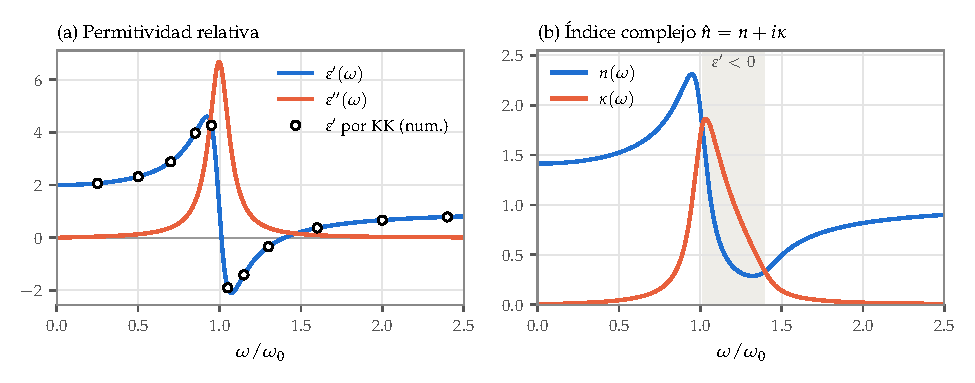
\includegraphics[width=\textwidth]{figuras/fig1_lorentz.pdf}
  \caption{Modelo de Lorentz con $\omega_p=\omega_0$ y $\gamma=0.15\,\omega_0$.
  (a) Partes real e imaginaria de $\eps$; los círculos son $\eps'$ reconstruida
  numéricamente a partir de $\eps''$ mediante la relación de Kramers--Kronig
  \eqref{eq:kkpos}. (b) Índice complejo; la franja gris marca la banda con
  $\eps'<0$.}
  \label{fig:lorentz}
\end{figure}

% ------------------------- Figura 2 ----------------------------------
\begin{figure}[t]
  \centering
  \tikzset{
    eje/.style={-{Stealth[length=5pt]},black!75,line width=0.5pt},
    flecha/.style={postaction={decorate},decoration={markings,
      mark=at position #1 with {\arrow{Stealth[length=5pt]}}}},
    polo/.style={font=\large}
  }
  \begin{subfigure}[b]{0.46\textwidth}
    \centering
    \begin{tikzpicture}[scale=1.25]
      % ejes
      \draw[eje] (-1.4,0) -- (1.6,0) node[right] {$\Re\omega$};
      \draw[eje] (0,-1.3) -- (0,1.45) node[above] {$\Im\omega$};
      % eje real recorrido
      \draw[black,line width=0.7pt,flecha=0.45] (-1.1,0) -- (1.1,0);
      % C+ (t<0)
      \draw[azul,dashed,line width=0.7pt,flecha=0.5] (1.1,0) arc (0:180:1.1);
      \node[azul,font=\small] at (0.85,0.95) {$C_+$};
      \node[azul,font=\small] at (-1.55,1.0) {$t<0$: sin polos};
      % C- (t>0)
      \draw[naranja,line width=0.7pt,flecha=0.5] (1.1,0) arc (0:-180:1.1);
      \node[naranja,font=\small] at (0.9,-0.95) {$C_-$};
      \node[naranja,font=\small] at (-1.1,-1.05) {$t>0$};
      % polos
      \node[polo] at (-0.62,-0.25) {$\times$};
      \node[polo] at ( 0.62,-0.25) {$\times$};
      \node[font=\small] at (-0.62,-0.48) {$\omega_-$};
      \node[font=\small] at ( 0.62,-0.48) {$\omega_+$};
    \end{tikzpicture}
    \caption{Respuesta impulsiva, ejemplo~\ref{ej:impulso}}
  \end{subfigure}\hfill
  \begin{subfigure}[b]{0.46\textwidth}
    \centering
    \begin{tikzpicture}[scale=1.25]
      \draw[eje] (-1.4,0) -- (1.6,0) node[right] {$\Re\omega'$};
      \draw[eje] (0,-1.3) -- (0,1.45) node[above] {$\Im\omega'$};
      % eje con indentación en omega=0.4
      \draw[black,line width=0.7pt,flecha=0.5] (-1.1,0) -- (0.3,0);
      \draw[black,line width=0.7pt] (0.5,0) arc (0:180:0.1);
      \draw[black,line width=0.7pt] (0.5,0) -- (1.1,0);
      \fill (0.4,0) circle (0.6pt);
      \node[font=\scriptsize] at (0.4,0.27) {$\gamma_\delta$};
      \node[font=\small] at (0.4,-0.2) {$\omega$};
      % C_R
      \draw[azul,line width=0.7pt,flecha=0.5] (1.1,0) arc (0:180:1.1);
      \node[azul,font=\small] at (0.95,0.95) {$C_R$};
      % polos de chi
      \node[polo] at (-0.6,-0.28) {$\times$};
      \node[polo] at ( 0.8,-0.32) {$\times$};
      \node[black!60,font=\small] at (-0.85,-0.62) {polos de $\chi$};
    \end{tikzpicture}
    \caption{Contorno para Kramers--Kronig}
  \end{subfigure}
  \caption{Contornos de integración. (a) Plano de la frecuencia: los polos
  $\omega_\pm$ del modelo de Lorentz están en el semiplano inferior, así que el
  contorno superior no encierra nada. (b) Contorno con indentación
  $\gamma_\delta$ sobre el punto $\omega'=\omega$; en su interior $\chi$ es
  analítica.}
  \label{fig:contornos}
\end{figure}

% =====================================================================
\section{Causalidad y relaciones de Kramers--Kronig}\label{sec:kk}

\subsection{De la causalidad a la analiticidad}

El ejemplo~\ref{ej:impulso} no depende del modelo de Lorentz. En cualquier
medio causal $\chi(t)=0$ para $t<0$, de modo que
$\chi(\omega)=\int_0^\infty\chi(t)\,e^{i\omega t}\,\dd t$. Si
$\omega=\omega_1+i\omega_2$ con $\omega_2>0$, el factor $e^{-\omega_2t}$ solo
mejora la convergencia y $\chi(\omega)$ resulta analítica en todo el semiplano
superior~\cite{Toll}. Además $\chi\to0$ cuando $|\omega|\to\infty$, porque a
frecuencias muy altas las cargas no alcanzan a seguir al campo; en el modelo
de Lorentz, $\chi\simeq-\omega_p^2/\omega^2$.

\subsection{Deducción con el teorema de los residuos}

Fijemos $\omega$ real e integremos $\chi(\omega')/(\omega'-\omega)$ sobre el
contorno de la figura~\ref{fig:contornos}b. No hay singularidades en su
interior, así que la integral total es cero; el arco $C_R$ no contribuye
porque el integrando decae más rápido que $1/|\omega'|$, y la indentación
aporta $-i\pi\chi(\omega)$ según la sección~\ref{sec:vp}. Queda
\begin{equation}\label{eq:kkcompleja}
  \vp\!\int_{-\infty}^{\infty}\frac{\chi(\omega')}{\omega'-\omega}\,\dd\omega'
  -i\pi\chi(\omega)=0
  \quad\Longrightarrow\quad
  \chi(\omega)=\frac{1}{i\pi}\,\vp\!\int_{-\infty}^{\infty}
  \frac{\chi(\omega')}{\omega'-\omega}\,\dd\omega'.
\end{equation}
Separando partes real e imaginaria:
\begin{equation}\label{eq:kk}
  \chi'(\omega)=\frac{1}{\pi}\,\vp\!\int_{-\infty}^{\infty}
  \frac{\chi''(\omega')}{\omega'-\omega}\,\dd\omega',\qquad
  \chi''(\omega)=-\frac{1}{\pi}\,\vp\!\int_{-\infty}^{\infty}
  \frac{\chi'(\omega')}{\omega'-\omega}\,\dd\omega'.
\end{equation}
Las partes real e imaginaria de una respuesta causal son, por tanto,
transformadas de Hilbert una de la otra: no son independientes. Como $\chi(t)$
es real, $\chi(-\omega)=\chi^*(\omega)$, es decir, $\chi'$ es par y $\chi''$
impar. Esto permite escribir las relaciones solo con frecuencias positivas, que
son las que se miden:
\begin{equation}\label{eq:kkpos}
  \eps'(\omega)-1=\frac{2}{\pi}\,\vp\!\int_0^\infty
  \frac{\omega'\eps''(\omega')}{\omega'^2-\omega^2}\,\dd\omega',\qquad
  \eps''(\omega)=-\frac{2\omega}{\pi}\,\vp\!\int_0^\infty
  \frac{\eps'(\omega')-1}{\omega'^2-\omega^2}\,\dd\omega'.
\end{equation}
Puede mostrarse que en un medio pasivo $\eps$ no se anula en el semiplano
superior, por lo que $\nh=\sqrt{\eps}$ también es analítica allí y tiende a 1.
Con $\alpha=2\omega\kappa/c$ se obtiene la forma más usada en óptica:
\begin{equation}\label{eq:kkn}
  n(\omega)-1=\frac{c}{\pi}\,\vp\!\int_0^\infty
  \frac{\alpha(\omega')}{\omega'^2-\omega^2}\,\dd\omega'.
\end{equation}
Basta medir la absorción en un rango espectral amplio para conocer el índice
de refracción. Este es el mismo tipo de relación que Kronig obtuvo para los
rayos~X~\cite{Kronig}. En la práctica, las colas del espectro que no se miden
deben extrapolarse; sobre el papel exacto de la causalidad puede
verse~\cite{Bechhoefer}.

\begin{ejemplo}{relajación de Debye}
Las moléculas polares de un líquido como el agua responden a un campo de
microondas con una susceptibilidad aproximada $\chi(\omega)=\chi_0/(1-i\omega\tau)$,
cuyo único polo, $\omega=-i/\tau$, está en el semiplano inferior (respuesta
$\chi(t)=(\chi_0/\tau)e^{-t/\tau}$ para $t>0$). Sus partes son
$\chi'=\chi_0/(1+\omega^2\tau^2)$ y $\chi''=\chi_0\omega\tau/(1+\omega^2\tau^2)$.
Verifiquemos la primera de~\eqref{eq:kk} calculando
$J=\vp\!\int\chi''(x)/(x-\omega)\,\dd x$ con~\eqref{eq:vp}. La función
$g(z)=\chi_0\tau z/[(1+\tau^2z^2)(z-\omega)]$ decae como $1/z^2$ y tiene un
polo en el semiplano superior, $z=i/\tau$, y uno sobre el eje, $z=\omega$:
\[
  \Res(g,i/\tau)=\frac{\chi_0}{2(i-\omega\tau)},\qquad
  \Res(g,\omega)=\frac{\chi_0\,\omega\tau}{1+\omega^2\tau^2}.
\]
Entonces
$J=\dfrac{i\pi\chi_0}{i-\omega\tau}+\dfrac{i\pi\chi_0\,\omega\tau}{1+\omega^2\tau^2}
=\dfrac{\pi\chi_0-i\pi\chi_0\,\omega\tau}{1+\omega^2\tau^2}
+\dfrac{i\pi\chi_0\,\omega\tau}{1+\omega^2\tau^2}
=\dfrac{\pi\chi_0}{1+\omega^2\tau^2}$, y en efecto $J/\pi=\chi'(\omega)$.
\end{ejemplo}

\subsection{Consecuencias: reglas de suma}

Las relaciones~\eqref{eq:kkpos} implican restricciones globales. A frecuencias
mucho mayores que todas las resonancias, la primera se reduce a
$\eps'-1\simeq-(2/\pi\omega^2)\int_0^\infty\omega'\eps''\,\dd\omega'$, y
comparando con $\eps'-1\simeq-\omega_p^2/\omega^2$ se obtiene la \emph{regla
de suma}
\begin{equation}\label{eq:regla}
  \int_0^\infty\omega\,\eps''(\omega)\,\dd\omega
  =\frac{\pi}{2}\,\omega_p^2=\frac{\pi Ne^2}{2\eps_0 m}.
\end{equation}
La absorción total, pesada por la frecuencia, depende solo de la densidad de
electrones y no de la forma de las resonancias. En el límite estático,
$\eps'(0)-1=(2/\pi)\int_0^\infty\eps''(\omega')/\omega'\,\dd\omega'$: un
material solo puede polarizarse en campos estáticos si absorbe en alguna
frecuencia. Para los parámetros de la figura~\ref{fig:lorentz}, la integral
numérica de~\eqref{eq:regla} da $1.570796$, igual a $\pi/2$; y los valores de
$\eps'$ reconstruidos con~\eqref{eq:kkpos} (círculos) coinciden con la curva
exacta con un error menor que $10^{-8}$.

% =====================================================================
\section{Interfaces: ley de Snell compleja y coeficientes de Fresnel}\label{sec:interfaces}

\subsection{Ley de Snell con índice complejo}

Una onda plana incide desde un medio transparente de índice $n_1$, con ángulo
$\theta_1$, sobre un medio de permitividad $\eps_2$. La continuidad de las
componentes tangenciales de $\mathbf{E}$ y $\mathbf{H}$ en todo punto de la
interfaz $z=0$ exige que la componente tangencial del vector de onda sea la
misma en los tres campos:
\begin{equation}\label{eq:snell}
  k_x=k_0n_1\sin\theta_1=k_0\nh_2\sin\hat\theta_2,\qquad
  \kh_{z2}=k_0\sqrt{\eps_2-n_1^2\sin^2\theta_1},\qquad
  \Im\kh_{z2}\ge0,
\end{equation}
con $k_0=\omega/c$. Si $\nh_2$ es complejo, el ``ángulo'' $\hat\theta_2$
también lo es y deja de ser un ángulo geométrico. Lo que tiene sentido físico
es el vector de onda transmitido $(k_x,0,\kh_{z2})$. Los planos de amplitud
constante son $z=\text{cte}$, mientras que los de fase constante son
$k_xx+\Re(\kh_{z2})z=\text{cte}$. Como no son paralelos, la onda transmitida es
\emph{inhomogénea}.

\subsection{Coeficientes de Fresnel}

Imponiendo las condiciones de frontera para las polarizaciones $s$ (TE) y $p$
(TM), con $k_{zj}=k_0\sqrt{\eps_j-n_1^2\sin^2\theta_1}$, se obtiene
\begin{equation}\label{eq:fresnel}
  r_s=\frac{k_{z1}-k_{z2}}{k_{z1}+k_{z2}},\qquad
  r_p=\frac{\eps_2k_{z1}-\eps_1k_{z2}}{\eps_2k_{z1}+\eps_1k_{z2}},\qquad
  t_s=\frac{2k_{z1}}{k_{z1}+k_{z2}},
\end{equation}
donde $r_p$ se refiere al cociente de campos magnéticos. Las mismas fórmulas
sirven para medios reales y absorbentes; basta usar la raíz con
$\Im k_{z2}\ge0$. A incidencia normal desde el aire,
$R=|(\nh-1)/(\nh+1)|^2=[(n-1)^2+\kappa^2]/[(n+1)^2+\kappa^2]$: un $\kappa$
grande produce una reflectancia cercana a 1, que es la razón por la que los
metales brillan.

\begin{ejemplo}{oro a 632.8\,nm}\label{ej:oro}
Interpolando linealmente los datos de Johnson y Christy~\cite{JohnsonChristy}
entre 616.8 y 659.5\,nm resulta $\nh\approx0.184+3.431i$, es decir,
$\eps\approx-11.74+1.26i$. Los valores publicados para el oro varían algo
según la preparación de la muestra~\cite{Olmon}, así que conviene tomar estas
cifras como representativas. Con~\eqref{eq:beer},
$\alpha=4\pi\kappa/\lambda_0=6.8\times10^{7}\,\mathrm{m^{-1}}$: la intensidad
cae a $1/e$ en solo 14.7\,nm. A incidencia normal, $R=0.944$.

Ahora la luz incide a $\theta_1=45^\circ$ desde el aire. Por~\eqref{eq:snell},
$\kh_{z2}/k_0=\sqrt{\eps-\tfrac12}=0.180+3.503i$. El campo decae como
$e^{-3.503\,k_0z}$, con longitud de $1/e$ igual a 28.7\,nm, mientras que la
fase avanza en la dirección $(\sin45^\circ,\,0.180)$, a $75.7^\circ$ de la
normal. En cambio, el ángulo complejo de Snell,
$\hat\theta_2=\arcsin(\sin\theta_1/\nh_2)\approx0.0108-0.204i$\,rad, tiene una
parte real de apenas $0.6^\circ$: no se puede leer como una dirección de
propagación. Con~\eqref{eq:fresnel}, $R_s=|r_s|^2=0.961$ y $R_p=|r_p|^2=0.924$.
\end{ejemplo}

\subsection{Reflexión total interna y onda evanescente}

Si $n_1>n_2$ (ambos reales) y $\theta_1$ supera el ángulo crítico
$\theta_c=\arcsin(n_2/n_1)$, el radicando de $k_{z2}$ se vuelve negativo y
$k_{z2}=i\,k_0\sqrt{n_1^2\sin^2\theta_1-n_2^2}$ es imaginario puro. Entonces
$|r_s|=|r_p|=1$ (la reflexión es total y solo cambia la fase), y en el segundo
medio hay un campo \emph{evanescente} que viaja a lo largo de la interfaz y
decae como $e^{-z/d_p}$, con
\begin{equation}\label{eq:dp}
  d_p=\frac{\lambda_0}{2\pi\sqrt{n_1^2\sin^2\theta_1-n_2^2}}.
\end{equation}
En promedio, la onda evanescente no transporta energía hacia el segundo medio.

\subsection{Reflexión total interna atenuada (ATR)}

Si el segundo medio absorbe, $\nh_2=n_2+i\kappa_2$, entonces $\kh_{z2}$
adquiere una parte real, aparece un flujo de energía hacia la muestra y
$|r|<1$: la reflexión total queda ``atenuada''. Este es el principio de la
espectroscopía ATR~\cite{Harrick,Fahrenfort}. La muestra se apoya contra un
cristal de índice alto y, al registrar $R(\lambda)$, se obtiene su espectro de
absorción. Solo se explora una capa de espesor del orden de $d_p$, de modo que
no hace falta preparar películas delgadas.

\begin{ejemplo}{profundidad de sondeo en ATR infrarroja}
Consideremos un cristal con $n_1\approx2.4$ (ZnSe o diamante en el
infrarrojo), $\theta_1=45^\circ$ y una muestra orgánica con $n_2\approx1.5$.
El ángulo crítico es $\theta_c=38.7^\circ$, así que hay reflexión total.
Con~\eqref{eq:dp}, $d_p=2.0\,\mu$m para $\lambda_0=10\,\mu$m
($1000\,\mathrm{cm^{-1}}$) y $d_p=1.0\,\mu$m para $\lambda_0=5\,\mu$m. Con un
cristal de germanio ($n_1\approx4.0$), a $10\,\mu$m, $d_p=0.66\,\mu$m. Como
$d_p\propto\lambda_0$, las bandas de longitud de onda larga se ven reforzadas
respecto de un espectro de transmisión, y por eso los espectros ATR suelen
corregirse antes de compararlos.
\end{ejemplo}

% =====================================================================
\section{Plasmónica de superficie: un polo del coeficiente de reflexión}\label{sec:spp}

\subsection{El plasmón como polo}

Un polo de $r_p$ significa una onda reflejada finita sin onda incidente, es
decir, un \emph{modo propio} de la interfaz. Para un dieléctrico $\eps_d$ sobre
un metal $\eps_m$, el denominador de~\eqref{eq:fresnel} se anula cuando
$\eps_mk_{zd}+\eps_dk_{zm}=0$. Usando $k_{zj}^2=\eps_jk_0^2-k_x^2$, se obtiene
la relación de dispersión del plasmón-polaritón de superficie (SPP):
\begin{equation}\label{eq:spp}
  k_{sp}=k_0\sqrt{\frac{\eps_m\eps_d}{\eps_m+\eps_d}}.
\end{equation}
Para que el modo esté ligado, ambos $k_{zj}$ deben ser imaginarios con parte
imaginaria positiva, lo que exige $\eps_m'<-\eps_d$. Esto ocurre en los metales
por debajo de su frecuencia de plasma. Conviene notar que entre dos
dieléctricos la misma expresión no da un polo sino un \emph{cero} de $r_p$: el
ángulo de Brewster, $\tan\theta_B=n_2/n_1$. Con el modelo de Drude sin
pérdidas, $\eps_m=-\eps_d$ ocurre en $\omega_{sp}=\omega_p/\sqrt{1+\eps_d}$, la
frecuencia límite del plasmón. Si el metal absorbe, el polo se aleja del eje
real de $k_x$: el modo se propaga una distancia $L=1/(2\Im k_{sp})$. Cuando una
fuente localizada excita la interfaz, su campo es una integral sobre $k_x$; al
deformar el contorno, el residuo en $k_x=k_{sp}$ da exactamente la onda
superficial $\propto e^{ik_{sp}x}$. Es el mismo mecanismo que encontró
Sommerfeld para las ondas de radio~\cite{Sommerfeld}.

\begin{ejemplo}{plasmón en oro a 632.8\,nm}
Con $\eps_m=-11.74+1.26i$ y~\eqref{eq:spp}:
\begin{itemize}
  \item \emph{Oro/aire} ($\eps_d=1$): $k_{sp}/k_0=1.0449+0.0052i$. El SPP se
  propaga $L=9.8\,\mu$m, penetra 332\,nm en el aire y solo 28\,nm en el metal.
  \item \emph{Oro/agua} ($\eps_d=1.332^2$): $k_{sp}/k_0=1.444+0.0136i$,
  $L=3.7\,\mu$m, y penetra 180\,nm en el agua.
\end{itemize}
Como $\Re k_{sp}>k_0\sqrt{\eps_d}$, la luz que llega desde el propio
dieléctrico nunca tiene suficiente $k_x$ para excitarlo. Ese desajuste de
momento es la razón por la que se usan prismas.
\end{ejemplo}

% ------------------------- Figura 3 ----------------------------------
\begin{figure}[t]
  \centering
  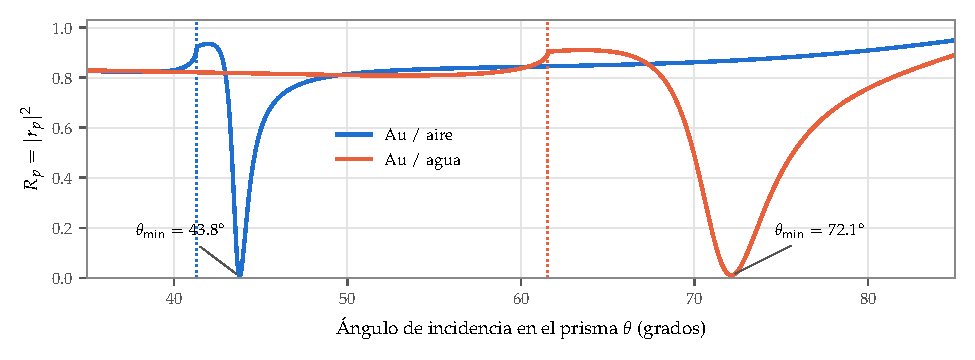
\includegraphics[width=\textwidth]{figuras/fig3_kretschmann.pdf}
  \caption{Reflectancia $p$ en la configuración de Kretschmann (prisma BK7,
  50\,nm de oro, $\lambda_0=632.8$\,nm), calculada con~\eqref{eq:airy}. Las
  líneas punteadas marcan el ángulo crítico de cada dieléctrico: sin la
  película de oro, por encima de ese ángulo la reflexión sería total. El mínimo
  pronunciado es la firma del polo de $r_p$ asociado al plasmón.}
  \label{fig:kretschmann}
\end{figure}

\subsection{Excitación en la configuración de Kretschmann}

En la configuración de Kretschmann y Raether~\cite{Kretschmann}, una película
metálica delgada se deposita sobre un prisma de índice $n_P$. La onda
evanescente de la reflexión total aporta $k_x=k_0n_P\sin\theta$, que puede
igualar a $\Re k_{sp}$. La reflectancia del sistema prisma/metal/dieléctrico se
calcula sumando las reflexiones múltiples en la película de espesor $d$
(fórmula de Airy):
\begin{equation}\label{eq:airy}
  r=\frac{r_{12}+r_{23}\,e^{2i\kh_{z2}d}}{1+r_{12}\,r_{23}\,e^{2i\kh_{z2}d}},
\end{equation}
donde cada $r_{ij}$ es el $r_p$ de~\eqref{eq:fresnel}. La
figura~\ref{fig:kretschmann} muestra el resultado para un prisma BK7
($n_P=1.515$) y 50\,nm de oro. La condición $n_P\sin\theta=\Re(k_{sp}/k_0)$
predice $43.6^\circ$ (aire) y $72.4^\circ$ (agua), y el cálculo completo da
mínimos casi nulos en $43.8^\circ$ y $72.1^\circ$. La pequeña diferencia se
debe a que el prisma perturba el modo, que ahora puede radiar hacia él. Si el
índice del agua pasa de 1.332 a 1.342, el mínimo se desplaza unos $1.5^\circ$,
es decir, $\approx150^\circ$ por unidad de índice. En esa sensibilidad, junto
con la penetración de unos 180\,nm del campo en la muestra, se basan los
biosensores SPR~\cite{Homola}.

% =====================================================================
\section{Conclusiones}

\begin{itemize}
  \item En un medio disipativo, $\eps$, $\nh$ y $\kh$ son complejos: $n$
  gobierna la refracción y $\kappa$ la absorción (ley de Beer--Lambert).
  \item El teorema de los residuos convierte las integrales de dispersión en
  sumas sobre polos, y la posición de esos polos tiene significado físico: en
  la frecuencia, el semiplano inferior expresa causalidad y amortiguamiento;
  en el número de onda, la absorción elige las ondas salientes.
  \item La causalidad hace a $\chi(\omega)$ analítica en el semiplano
  superior; un contorno indentado da las relaciones de Kramers--Kronig, que
  ligan refracción y absorción, y la regla de suma~\eqref{eq:regla}.
  \item Con índice complejo, la ley de Snell sigue siendo la conservación de
  $k_x$, pero el ángulo de refracción pierde su sentido geométrico. La
  reflexión total interna crea ondas evanescentes que, sobre una muestra
  absorbente, producen la ATR, y sobre un metal, a través de un polo de $r_p$,
  el plasmón de superficie.
\end{itemize}

% =====================================================================
\renewcommand{\refname}{\color{azul}Bibliografía}
\begin{thebibliography}{99}
\footnotesize
\setlength{\itemsep}{0pt}

\bibitem{Jackson} J.~D. Jackson, \emph{Classical Electrodynamics}, 3.ª ed.
(Wiley, Nueva York, 1999).

\bibitem{BornWolf} M.~Born y E.~Wolf, \emph{Principles of Optics}, 7.ª ed.
(Cambridge University Press, 1999).

\bibitem{Arfken} G.~B. Arfken, H.~J. Weber y F.~E. Harris, \emph{Mathematical
Methods for Physicists}, 7.ª ed. (Academic Press, 2013).

\bibitem{Sommerfeld} A.~Sommerfeld, ``Über die Ausbreitung der Wellen in der
drahtlosen Telegraphie'', Ann. Phys. (4) \textbf{28}, 665--736 (1909).

\bibitem{Kronig} R.~de L. Kronig, ``On the theory of dispersion of X-rays'',
J. Opt. Soc. Am. \textbf{12}, 547--557 (1926).
\href{https://doi.org/10.1364/JOSA.12.000547}{doi:10.1364/JOSA.12.000547}

\bibitem{Kramers} H.~A. Kramers, ``La diffusion de la lumière par les
atomes'', \emph{Atti del Congresso Internazionale dei Fisici}, Como, vol.~2,
545--557 (1927).

\bibitem{Toll} J.~S. Toll, ``Causality and the dispersion relation: logical
foundations'', Phys. Rev. \textbf{104}, 1760--1770 (1956).
\href{https://doi.org/10.1103/PhysRev.104.1760}{doi:10.1103/PhysRev.104.1760}

\bibitem{Bohren} C.~F. Bohren, ``What did Kramers and Kronig do and how did
they do it?'', Eur. J. Phys. \textbf{31}, 573--577 (2010).
\href{https://doi.org/10.1088/0143-0807/31/3/014}{doi:10.1088/0143-0807/31/3/014}

\bibitem{Harrick} N.~J. Harrick, ``Surface chemistry from spectral analysis of
totally internally reflected radiation'', J. Phys. Chem. \textbf{64},
1110--1114 (1960).
\href{https://doi.org/10.1021/j100838a005}{doi:10.1021/j100838a005}

\bibitem{Fahrenfort} J.~Fahrenfort, ``Attenuated total reflection: a new
principle for the production of useful infra-red reflection spectra of organic
compounds'', Spectrochim. Acta \textbf{17}, 698--709 (1961).
\href{https://doi.org/10.1016/0371-1951(61)80136-7}{doi:10.1016/0371-1951(61)80136-7}

\bibitem{Ritchie} R.~H. Ritchie, ``Plasma losses by fast electrons in thin
films'', Phys. Rev. \textbf{106}, 874--881 (1957).
\href{https://doi.org/10.1103/PhysRev.106.874}{doi:10.1103/PhysRev.106.874}

\bibitem{Otto} A.~Otto, ``Excitation of nonradiative surface plasma waves in
silver by the method of frustrated total reflection'', Z. Phys. \textbf{216},
398--410 (1968).
\href{https://doi.org/10.1007/BF01391532}{doi:10.1007/BF01391532}

\bibitem{Kretschmann} E.~Kretschmann y H.~Raether, ``Radiative decay of non
radiative surface plasmons excited by light'', Z. Naturforsch. A \textbf{23},
2135--2136 (1968).
\href{https://doi.org/10.1515/zna-1968-1247}{doi:10.1515/zna-1968-1247}

\bibitem{Homola} J.~Homola, S.~S. Yee y G.~Gauglitz, ``Surface plasmon
resonance sensors: review'', Sens. Actuators B \textbf{54}, 3--15 (1999).
\href{https://doi.org/10.1016/S0925-4005(98)00321-9}{doi:10.1016/S0925-4005(98)00321-9}

\bibitem{Barnes} W.~L. Barnes, A.~Dereux y T.~W. Ebbesen, ``Surface plasmon
subwavelength optics'', Nature \textbf{424}, 824--830 (2003).
\href{https://doi.org/10.1038/nature01937}{doi:10.1038/nature01937}

\bibitem{Zayats} A.~V. Zayats, I.~I. Smolyaninov y A.~A. Maradudin,
``Nano-optics of surface plasmon polaritons'', Phys. Rep. \textbf{408},
131--314 (2005).
\href{https://doi.org/10.1016/j.physrep.2004.11.001}{doi:10.1016/j.physrep.2004.11.001}

\bibitem{Bechhoefer} J.~Bechhoefer, ``Kramers--Kronig, Bode, and the meaning
of zero'', Am. J. Phys. \textbf{79}, 1053 (2011).
\href{https://doi.org/10.1119/1.3614039}{doi:10.1119/1.3614039}

\bibitem{JohnsonChristy} P.~B. Johnson y R.~W. Christy, ``Optical constants of
the noble metals'', Phys. Rev. B \textbf{6}, 4370--4379 (1972).
\href{https://doi.org/10.1103/PhysRevB.6.4370}{doi:10.1103/PhysRevB.6.4370}

\bibitem{Olmon} R.~L. Olmon \emph{et al.}, ``Optical dielectric function of
gold'', Phys. Rev. B \textbf{86}, 235147 (2012).
\href{https://doi.org/10.1103/PhysRevB.86.235147}{doi:10.1103/PhysRevB.86.235147}

\end{thebibliography}

\end{document}
